\documentclass[../TDAM3.tex]{subfiles}%

\begin{document}
\section{Alliages du cuivre}
\enonce{%
	Le cuivre peut être utilisé pur, notamment pour des applications exploitant sa
	haute conductivité électrique, ou bien en alliage tels que le laiton (alliage
	cuivre-zinc) et le bronze (cuivre-étain).
	\begin{tcn}(defi)<lftt>'l'{Données}
		\begin{itemize}[]
			\item $\rho_{\ce{Cu}} = \SI{8.96e3}{kg.m ^{-3}}$~;
			\item $M_{\ce{Cu}} = \SI{63.5}{g.mol^{-1}}$~; $M_{\ce{Ag}} =
				      \SI{108}{g.mol^{-1}}$~; $M_{\ce{Zn}} = \SI{65.4}{g.mol^{-1}}$~;
			\item $r_{\ce{Cu}} = \SI{128}{pm}$~; $r_{\ce{Ag}} = \SI{144}{pm}$~;
			      $r_{\ce{Zn}} = \SI{134}{pm}$.
		\end{itemize}
	\end{tcn}
}%
\QR{%
	Le cuivre pur cristallins dans un réseau CFC. Représenter la maille et
	déterminer sa population. Déterminer le paramètre de maille $a$.
}{%
	Voir cours~: $N = 8\times1/8 + 6\times1/2 = 4$. Dans une maille CFC, il
	y a contact le long de la diagonale d'une face~; ainsi,
	\[
		a \sqrt{2} = 4r_{\ce{Cu}}
		\qqdonc
		\boxed{a = \frac{4r_{\ce{Cu}}}{\sqrt{2}} = \SI{361}{pm}}
	\]
	% TODO: schéma exercice
}%

\enonce{%
	Lorsqu'un atome a un rayon voisin de celui du cuivre, il peut former des
	alliages dits de substitution, où l'hétéroatome remplace un pour plusieurs
	atomes de cuivres par maille.
}%

\begin{blocQR}
	\item \enonce{%
		L'alliage \ce{Cu}-\ce{Ag} est utilisé pour augmenter la résistance à la
		température du matériau. Dans cette structure, les atomes d'argent
		remplacent les atomes de cuivre aux sommets de la maille.
	}%

	\QR{%
		Faire un schéma de la maille. Quelle est la stœchiométrie de
		l'alliage~?
	}{%
		Schéma à faire. La maille compte $8\times1/8 = 1$ atome d'argent, et
		$6\times1/2 = 3$ atomes de cuivre~; l'alliage est donc \fbox{\ce{Cu_3Ag}}.
	}%
	\QR{%
	Déterminer le nouveau paramètre de maille $a'$ ainsi que la masse
	volumique $\rho'$ de l'alliage. Commenter.
	}{%
	Contact entre atomes le long de la diagonale d'une face, donc
	\[
		a' \sqrt{2} = 2r_{\ce{Cu}} + 2r_{\ce{Ag}}
		\qqdonc
		\boxed{a' = \SI{385}{pm} > a}
	\]
	ce qui est logique puisque le rayon métallique de l'argent est supérieur
	à celui du cuivre. La masse volumique vaut
	\[
		\boxed{\rho' = \frac{3M_{\ce{Cu}} + M_{\ce{Ag}}}{\Nc_A a'^{3}} =
		\SI{8.71e3}{kg.m^{-3}}}
	\]
	}%
	\item \enonce{%
		Le laiton, alliage \ce{Cu}-\ce{Zn}, est l'alliage le plus fabriqué. Il
		permet d'augmenter la résistance mécanique et la dureté du cuivre, mais
		diminue la densité et la conductivité thermique. La structure du laiton peut
		être décrite par un réseau cubique hôte d'atomes de cuivres avec un atome de
		zinc au centre du cube.
	}%
	\QR{%
		Faire un schéma de la maille. Quelle est la stœchiométrie de
		l'alliage~?
	}{%
		Voir figure. On compte $8\times1/8 = 1$ atome de cuivre par maille,
		et 1 atome de zinc, d'où \fbox{\ce{CuZn}}.
		\begin{figure}[h]
			\centering
			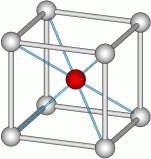
\includegraphics[scale=1]{laiton}
			\caption{Maille élémentaire du laiton. Le cuivre est en gris, l'atome
				de zinc en rouge.}
			\label{fig:laiton}
		\end{figure}
	}%

	\QR{%
	Déterminer le nouveau paramètre de maille $a''$ ainsi que la masse
	volumique $\rho''$ de l'alliage.
	}{%
	Contact le long de la grande diagonale~:
	\[
		a'' \sqrt{3} = 2r_{\ce{Cu}} + 2r_{\ce{Zn}}
		\qqdonc
		\boxed{a'' = \SI{303}{pm}}
	\]
	et la masse volumique vaut
	\[
		\boxed{\rho'' = \frac{M_{\ce{Cu}} + M_{\ce{Zn}}}{\Nc_Aa''^{3}} = \SI{7.71e3}{kg.m ^{-3}}}
	\]
	}%

\end{blocQR}


\QR{%
	Les différences structurales induites par la substitution sont
	responsables d'une modification des propriétés de conduction électrique et
	de résistance mécanique. Proposer une explication.
}{%
	On constate à partir des résultats précédents que les mailles sont
	déformées dans les alliages. Ceci a un effet sur la facilité de
	déplacement des électrons de conduction au sein du cristal, et donc sur ses
	propriétés de conduction électrique macroscopique. La présence
	d'hétéroélements rend plus difficile le glissement des plans de cations les
	uns sur les autres dans le matériau, ce qui explique la modification des
	propriétés mécaniques.
}%

\end{document}
